%!TEX root = ../lections.tex

\begin{wrapfigure}[9]{l}{0.4\linewidth} 
\vspace{0.15em}
\centering
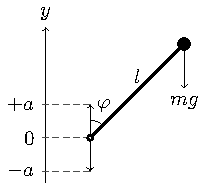
\includegraphics[scale=1.5]{img/kap_pendulum/kap_pendulum}
% \vspace{-0.25em}
% \caption{Some caption}
% \label{fig:somelabel}
\end{wrapfigure}
Рассмотрим шарик на упругом стержне, пренебрегая массой стержня. Точка подвеса колеблется с амплитудой $a$ и периодом $2\tau$. Изначально маятник расположен в верхнем положении равновесия. 


Пусть $\tau \ll 1$ (точка подвеса быстро осциллирует) и $l\gg a$.

Пусть точка подвеса совершает равнопеременные движения с ускорением $a \pm c$, тогда с каждым полупериодом $c=\frac{8a}{\tau^2}$, частота $\omega_p^2=\frac{c}{l}=\frac{8a}{l\tau^2}$. Считаем, что диссипации нет. 

Систему можно описать уравнениями:
\begin{equation}
	\left\{\begin{aligned}
		\dot{\varphi}=y \\
		\dot{y}=(\omega_0^2 \pm \omega_p^2)	\varphi,
	\end{aligned}\right.
	\label{eq:89}	
\end{equation}
где $\omega_0$ - собственная частота маятника, если бы не было колебаний подвеса. Знак $\pm$ изменяется через время $\tau$, $\omega_p^2>\omega_0^2$. Эта система параметрическая, к ней можно применить недавно рассмотренную теорию. 

Система  \eqref{eq:89} является кусочно-линейной. Построим матрицу $G$.

\paragraph{Матрица $G_1$.} Пусть в начальный момент точка подвеса в крайнем верхнем положении. Тогда в течение первого полупериода:
\begin{gather*}
	\dot{\varphi}=y,\quad
	\dot{y}=p^2\varphi,\quad
	p^2=\omega_0^2 + \omega_p^2.
\end{gather*}
$p$ действительные и разного знака. ФСР можно записать в виде:
\begin{gather}
	\phi_1(t)=\ch(pt),\quad \psi_1(t)=\frac1{p}\sh(pt), \notag \\ 
	\phi_2(t)=p\sh(pt),\quad \psi_2(t)=\ch(pt).		
	\label{eq:90}
\end{gather}
Тогда элементы матрицы будут
\begin{gather*}
	a_1=\ch(p\tau), c_1=\frac1{p}\sh(p\tau), \notag \\ 
	b_1=p\sh(p\tau), d_1=\ch(p\tau).		
\end{gather*}

\paragraph{Матрица $G_2$.} Будем считать, что маятник в нижнем положении и начинает движение вверх:
\begin{gather}
	\dot{\varphi}=y,\quad
	\dot{y}=p^2\varphi,\quad
	p^2=\omega_0^2 - \omega_p^2.
	\label{eq:91}
\end{gather}
Корни чисто мнимые. Фундаментальная система решений:
\begin{gather*}
	\phi_1(t)=\cos(\omega t),\quad \psi_1(t)=\frac1{\omega}\sin(\omega t), \notag \\ 
	\phi_2(t)=-\omega \sin(\omega t),\quad \psi_2(t)=\cos(\omega t).
\end{gather*}
Подставляя $\tau$, найдем:
\begin{gather*}
	a_1=\cos(\omega \tau), \quad c_1=\frac1{\omega}\sin(\omega \tau), \notag \\ 
	b_1=-\omega \sin(\omega \tau), \quad d_1=\cos(\omega \tau).		
\end{gather*}

Перемножаем $G_1 \cdot G_2$, получаем:
\begin{gather*}
	P=a+d=2\ch(p \tau)\cos(\omega \tau)+\qty(\frac{p}{\omega}-\frac{\omega}{p})\sh(p \tau)\sin(\omega \tau).		
\end{gather*}

Для устойчивости $|P|<1$. Получаем неравенство на параметры. Оно строилось численно, заданы: $a=0.1$см, $l=100$ см.

\begin{wrapfigure}[9]{l}{0.5\linewidth} 
	\vspace{0.1em}
	\centering
	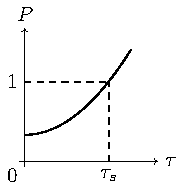
\includegraphics[scale=1.5]{img/kap_pendulum/p_tau}
	\vspace{-0.25em}
\end{wrapfigure}

Существует интервал, где неравенство выполняется. В данном случае $\tau_s=0.006738$. Число колебаний $N=\frac{1}{2\tau}$. Если $N>678$ колебаний в секунду, то верхняя точка становится устойчивой. Внешнее воздействие превратило неустойчивое состояние равновесия в высокочастотное колебание вблизи состояния равновесия.





\subsection{Колебания линейного осциллятора с медленно меняющейся частотой}
Рассмотрим линейный осциллятор:
\begin{gather}
	\ddot{x}+\omega_0^2(\mu t)x=0, \qq{где} \omega_0(\mu t)>0,~0< \mu \ll t
	\label{eq:92}
\end{gather}
Введём новое время $\tau=\mu t$, тогда
\begin{gather}
	\left\{\begin{aligned}
		&\mu \dv{x}{\tau}=y \\
		&\mu \dv{y}{\tau}=-\omega_0^2(\tau)x.
	\end{aligned}\right.	
	\label{eq:93}
\end{gather}
Для исследования используем метод Вентцеля-Крамерса-Бриллюэна (ВКБ). В соответствии с ним, будем искать решение в виде:
\begin{gather}
	\left\{\begin{aligned}
		x=e^{\frac{s(\tau)}{\mu}}\sum\limits_{j=0}^{\infty}\mu^j u_j(\tau) \\
		y=e^{\frac{s(\tau)}{\mu}}\sum\limits_{j=0}^{\infty}\mu^j v_j(\tau),
	\end{aligned}\right.	
	\label{eq:94}
\end{gather}
где $s(\tau),~u_j(\tau),~v_j(\tau)$ - неизвестные функции, которые надо найти. 

Будем искать решение нулевого порядка по $\mu$:
\begin{gather}
	\left\{\begin{aligned}
		x=e^{\frac{s(\tau)}{\mu}}\qty[u_0(\tau)+\mu u_1(\tau)] \\
		y=e^{\frac{s(\tau)}{\mu}}\qty[v_0(\tau)+\mu v_1(\tau)].
	\end{aligned}\right.	
	\label{eq:95}
\end{gather}
Подставляем \eqref{eq:95} в \eqref{eq:93} и группируем слагаемые по порядку $\mu$:
\begin{equation}
	\mu^0:
	\left\{\begin{aligned}
		&\dv{s}{\tau} u_0(\tau)-v_0(\tau)=0 \\
		&\omega^2_0(\tau)u_0(\tau)+\dv{s}{\tau} v_0(\tau)=0, 		
	\end{aligned}\right.
	\label{eq:96}	
\end{equation}
\begin{equation}
	\mu^1:
	\left\{\begin{aligned}
		&\dv{s}{\tau} u_1(\tau)+\dv{u_0}{\tau}=v_1(\tau) \\
		&\dv{s}{\tau} v_1(\tau)+\dv{v_0}{\tau}=-\omega^2_0(\tau)u_1(\tau). 		
	\end{aligned}\right.
	\label{eq:97}	
\end{equation}

Система \eqref{eq:96} представляет собой СЛАУ относительно $u_0$, $v_0$. Из условия равенства нулю определителя системы получим
\begin{equation}
	\qty(\dv{s}{\tau})^2+\omega^2_0(\tau)=0,
	\label{eq:98}	
\end{equation}
\begin{equation}
	\dv{s}{\tau}=\pm i\omega_0(\tau),
	\label{eq:99}	
\end{equation}

Проинтегрируем:
\begin{gather}
	s(\tau)=\pm i \int_0^{\tau}\omega_0(\tau)\dd \tau, \qq{тогда} ~u_0=\psi(\tau), ~v_0=\pm i \omega_0(\tau)\psi(\tau), 
	\label{eq:100}
\end{gather}
где $\psi(\tau)$ -- ввели произвольную функцию (просто переобозначили $u_0(\tau)$).

Уравнение \eqref{eq:100} определяет пару комплексно сопряженных решений. Рассмотрим с <<$+$>>:
\begin{equation}
	v_1(\tau)=\dv{s}{\tau}u_1(\tau)+\dv{\psi}{\tau}.
	\label{eq:101}	
\end{equation}
Подставляя \eqref{eq:100} и \eqref{eq:101} в \eqref{eq:97}, получим:
\begin{equation}
	2\omega_0(\tau)\dv{\psi}{\tau}=-\psi\dv{\omega_0(\tau)}{\tau}.
	\label{eq:102}	
\end{equation}
В \eqref{eq:102} переменные разделяются. Проинтегрируем:
\begin{equation*}
	\psi(\tau)=\frac{A}{\sqrt{\omega_0(\tau)}}.
\end{equation*}
Чтобы составить полное решение, нужно проделать ту же процедуру для знака <<$-$>>. В итоге получим
\begin{equation*}
	x(\tau) \approx \frac{A}{\sqrt{\omega_0(\tau)}} \exp \qty[\frac{i}{\mu}\int_0^{\tau}\omega_0(\tau)\dd \tau]+\frac{A}{\sqrt{\omega_0(\tau)}} \exp \qty[-\frac{i}{\mu}\int_0^{\tau}\omega_0(\tau)\dd \tau],
\end{equation*}
или, возвращаясь к исходному времени
\begin{gather}
	x(t) \approx \frac{2A}{\sqrt{\omega_0(\mu t)}}\cos\vartheta, \qq{где}
	\vartheta=\int_0^{\mu \tau}\omega_0(t)\dd t
	\label{eq:103s}
\end{gather}

Найдем полную энергию осциллятора:
\begin{equation}
	E=\frac{(\dot x)^2}{2}+\omega_0^2(\mu t)\frac{x^2}{2}, 
	\label{eq:104}
\end{equation}
\begin{equation}
	\dot{x}=-\frac{A\cos\vartheta \cdot \dot{\omega}(\mu t)}{\omega_0(\mu t)\sqrt{\omega_0(\mu t)}}-\frac{2A\sin\vartheta \cdot \omega_0(\mu t)}{\sqrt{\omega_0(\mu t)}}.
	\label{eq:105}	
\end{equation}
В первом приближении $\dot \omega \approx 0$, поэтому формула упрощается:
\begin{equation}
	\dot{x}=-2A\sqrt{\omega_0(\mu t)}\sin\vartheta.
	\label{eq:106}	
\end{equation}
Подставим \eqref{eq:103s}, \eqref{eq:106} в \eqref{eq:104}:
\begin{equation*}
	E \approx A^2 \omega_0(\mu t).
\end{equation*}
Энергия меняется пропорционально частоте изменения осциллятора:
\begin{equation*}
	\frac{E}{\omega_0(\mu t)}=const.
\end{equation*}

Увеличивая частоту, увеличиваем и энергию. А отношение их есть \textbf{адиабатический} (т.к. медленно меняем частоту) \textbf{инвариант}. 

Итак, мы рассмотрели линейные параметрические системы: резонансные (условия параметрического резонанса), быстро осциллирующие и медленно осциллирующие.
